\documentclass[../main.tex]{subfiles}

\begin{document}
\begin{questions}

\question Calculate the curl and divergence of the following vector functions. If the curl turns out to be zero, construct a scalar function $\phi$ of which the vector field is the gradient:
\begin{parts}
	\part $F_x = x + y$ ; $F_y = -x + y$ ; $F_z = -2z$
	\begin{solution}
		\begin{align}
			\vec{F}(x,y,z) &= (x+y,-x+y,-2z) \\
			\text{Curl: } \nabla \times \vec{F} &= 
				\begin{vmatrix}
					\hat{\imath} & \hat{\jmath} & \hat{k} \\
					\frac{\partial}{\partial x} & \frac{\partial}{\partial y} & \frac{\partial}{\partial z} \\
					x+y & -x+y & -2z
				\end{vmatrix}
				\\
			&= 0\hat{\imath} - 0\hat{\jmath} + (-1-1)\hat{k} = \boxed{-2\,\hat{k}} \\
			\text{Div: } \nabla \cdot \vec{F} &= \frac{\partial}{\partial x} (x+y) + \frac{\partial}{\partial y} (-x+y) + \frac{\partial}{\partial z} (-2z) \\
			&= 1 + 1 - 2 = \boxed{0} 
		\end{align}
	\end{solution}
	\part $G_x = 2y$ ; $G_y = 2x + 3z$ ; $G_z = 3y$
	\begin{solution}
		\begin{align}
			\vec{G}(x,y,z) &= (2y,2x+3z,3y) \\
			\text{Curl: } \nabla \times \vec{G} &= 
				\begin{vmatrix}
					\hat{\imath} & \hat{\jmath} & \hat{k} \\
					\frac{\partial}{\partial x} & \frac{\partial}{\partial y} & \frac{\partial}{\partial z} \\
					2y & 2x+3z & 3y
				\end{vmatrix}
				\\
			&= (3-3)\hat{\imath} - 0\hat{\jmath} + (2-2)\hat{k} = \boxed{\vec{0}} \\
			\text{Div: } \nabla \cdot \vec{G} &= \frac{\partial}{\partial x} (2y) + \frac{\partial}{\partial y} (2x+3z) + \frac{\partial}{\partial z} (3y) \\
			&= 0 + 0 + 0 = \boxed{0} \\
			\phi\text{: } G_x &= \frac{\partial}{\partial x}\phi(x,y,z) = 2y \\
			\implies \phi(x,y,z) &= 2xy + \psi(y,z) \\
			\implies \frac{\partial}{\partial y}\phi(x,y,z) &= 2x + \frac{\partial}{\partial y}\psi(y,z) = G_y = 2x + 3z \\
			\implies \frac{\partial}{\partial y}\psi(y,z) &= 3z \\
			\implies \psi(y,z) &= 3yz + \omega(z) \\
			\implies \phi(x,y,z) &= 2xy + 3yz + \omega(z) \\
			\implies \frac{\partial}{\partial z}\phi(x,y,z) &= 3y + \frac{\partial}{\partial z}\omega(z) \\
			\implies \omega(z) &= C \\
			\implies \phi(x,y,z) &= \boxed{2xy + 3yz + C}
		\end{align}
	\end{solution}
	\part $H_x = x^2 - z^2$ ; $H_y = 2$ ; $H_z = 2xz$
	\begin{solution}
		\begin{align}
			\vec{H}(x,y,z) &= (x^2-z^2,2,2xz) \\
			\text{Curl: } \nabla \times \vec{H} &= 
				\begin{vmatrix}
					\hat{\imath} & \hat{\jmath} & \hat{k} \\
					\frac{\partial}{\partial x} & \frac{\partial}{\partial y} & \frac{\partial}{\partial z} \\
					x^2-z^2 & 2 & 2xz
				\end{vmatrix}
				\\
			&= 0\hat{\imath} - (2z+2z)\hat{\jmath} + 0\hat{k} = \boxed{-4z\,\hat{\jmath}} \\
			\text{Div: } \nabla \cdot \vec{H} &= \frac{\partial}{\partial x} (x^2-y^2) + \frac{\partial}{\partial y} (2) + \frac{\partial}{\partial z} (2xz) \\
			&= 2x + 0 + 2x = \boxed{4x} 
			\end{align}
	\end{solution}
\end{parts}

\question Calculate the Laplacian of the following functions:
\begin{parts}
	\part $T_a = x^2 + 2xy + 3z + 4$
	\begin{solution}
		\begin{align}
			\nabla \cdot \nabla T_a &= \frac{\partial^2 T_a}{\partial x^2} + \frac{\partial ^2T_a}{\partial y^2} + \frac{\partial^2 T_a}{\partial z^2}\\
			&= 2+0+0\\
			&= \boxed{2}
		\end{align}
	\end{solution}
	\part $T_b = \sin(x) \sin(y) \sin(z)$
	\begin{solution}
		\begin{align}
			\nabla \cdot \nabla T_b &= \frac{\partial^2 T_b}{\partial x^2} + \frac{\partial ^2T_b}{\partial y^2} + \frac{\partial^2 T_b}{\partial z^2}\\
			&= \boxed{-3\sin(x) \sin(y) \sin(z)}\\
		\end{align}
	\end{solution}
	\part $T_c = e^{-5x}\sin(4y)\cos(3z)$
	\begin{solution}
		\begin{align}
			\nabla \cdot \nabla T_c &= \frac{\partial^2 T_c}{\partial x^2} + \frac{\partial ^2T_c}{\partial y^2} + \frac{\partial^2 T_c}{\partial z^2}\\
			&= 25e^{-5x}\sin(4y)\cos(3x)-16e^{-5x}\sin(4y)\cos(3x)\\
			&-9e^{-5x}\sin(4y)\cos(3x)\\
			&= \boxed{0}
		\end{align}
	\end{solution}
	\part $\vec{v} = x^2\,\ihat + 3xz^2\,\jhat - 2xz\,\khat$
	\begin{solution}
		\begin{align}
			\nabla^2 \vec{v} &= \nabla^2{v_x}\,\ihat + \nabla^2{v_y}\,\jhat + \nabla^2{v_z}\,\khat\\
			&= 2\,\ihat+6x\,\jhat
		\end{align}
	\end{solution}
\end{parts}

\question Test the Stokes' theorem for the vector field $\vec{v} = xy \hat{i} ~+~ 2yz \hat{j} ~+~  3z\hat{k}$ using a triangular area with vertices $(0,0,0)$, $(0,2,0)$ and $(0,0,2)$.

\begin{solution}
	\begin{center}
		\tdplotsetmaincoords{80}{45}
		\begin{tikzpicture}[tdplot_main_coords]
			\draw[thick,->] (0,0,0) -- (3,0,0) node[anchor=north west]{$x$};
			\draw[thick,->] (0,0,0) -- (0,3,0) node[anchor=north west]{$y$};
			\draw[thick,->] (0,0,0) -- (0,0,3) node[anchor=south]{$z$};

			\draw (0,0,0) node[anchor= north east]{(0,0,0)} -- (0,2,0) node[anchor= south west]{(0,2,0)} -- (0,0,2) node[anchor= east]{(0,0,2)} -- cycle;

			\begin{scope}[canvas is yz plane at x=0]
				\draw[->] (0.75,0.2) arc (-67.5:247.5:0.5) node[yshift=1.1cm, xshift=-0.1cm]{$\Gamma$};
			\end{scope}

			\draw[->] (0,0.56,0.66) -- (1.4,0.56,0.66) node[anchor=south]{$d\vec{S}$};

		\end{tikzpicture}
	\end{center}

	According to Stokes theorem:
	\begin{align}
		\oint_\Gamma \vec{v} \cdot d\vec{\Gamma} = \iint_S \nabla \times \vec{v} \cdot d\vec{S}
	\end{align}
	where
	\begin{description}
		\item[$\vec{v}$] is a vector field (given in our case)
		\item[$S$] is the surface (of the triangle) with a given orientation (defined by orientation of $\Gamma$)
		\item[$\Gamma$] is the boundary of the surface with a given orientation (orientation specified in figure)
	\end{description}
	Let us work on the RHS first. For that, we need $d\vec{S}$. We can simply observe that $d\vec{S}=dy\,dz\,\hat{\imath}$. But there might be more complicated surfaces in the future (or in your exams), so we need a more rigorous way of finding $d\vec{S}$. We can use our MA knowledge (existant or not) to parametrize the triangle surface as
	\begin{equation}
		\vec{r}\,(y,z) = 0\,\hat{\imath} + y\,\hat{\jmath} + z\,\hat{k};\,\, 0 \leq y \leq 2, \, 0 \leq z \leq 2-y
	\end{equation}
	This parametrization is very simple because our surface is really a part of the yz plane.
	Now $d\vec{S}=\vec{r_y}\times\vec{r_z}=(dy\,\hat{\jmath})\times(dz\,\hat{k})=dy\,dz\,\hat{\imath}$. Why did we choose $\vec{r_y}\times\vec{r_z}$ and not $\vec{r_z}\times\vec{r_y}$? Because the former leads to the orientation we want.
	Now since $d\vec{S}$ has only an $\hat{\imath}$ component, we only need the $\hat{\imath}$ component of $\nabla\times\vec{v}$, since it's being dotted with $d\vec{S}$ in the RHS.
	\begin{equation}
		(\nabla\times\vec{v})_{\hat{\imath}} = \frac{\partial}{\partial y}(3zk)-\frac{\partial}{\partial z}(2yz)=-2y
	\end{equation}
	\begin{align}
		\text{RHS}&=\int^{y=2}_{y=0}\int^{z=2-y}_{z=0}-2y\,dz\,dy \\
		&= -2\int^{y=2}_{y=0}2y-y^2\,dy \\
		&= -2(4-\frac{8}{3}) = -\frac{8}{3}
	\end{align}
	Now we need LHS. $\Gamma$ can be parametrized as
	\begin{gather}
		\vec{r_1}(t) = 0\,\hat{\imath} + t\,\hat{\jmath} + (2-t)\,\hat{k};\,\, 0 \leq t \leq 2 \implies d\vec{r_1}(t) = dt\,\hat{\jmath}-dt\,\hat{k} \\
		\vec{r_2}(t) = 0\,\hat{\imath} + 0\,\hat{\jmath} + t\,\hat{k};\,\, 0 \leq t \leq 2 \implies d\vec{r_2}(t) = dt\,\hat{k}\\
		\vec{r_3}(t) = 0\,\hat{\imath} + t\,\hat{\jmath} + 0\,\hat{k};\,\, 0 \leq t \leq 2 \implies d\vec{r_3}(t) = dt\,\hat{\jmath}
	\end{gather}
	Each of $\vec{r_1},\,\vec{r_2},\,\vec{r_3}$ is a parametrization of one side of the triangle.
	\begin{align}
		\text{LHS}&=\int^{0}_2\vec{v}\cdot(\hat{\jmath}-\hat{k})\,dt+\int^{0}_2\vec{v}\cdot\hat{k}\,dt+\int^{2}_0\vec{v}\cdot\hat{\jmath}\,dt \\
		&=\int^2_0v_z-v_y\,dt-\int^2_0v_z\,dt+\int^2_0v_y\,dt \\
		&=\int^2_03(2-t)k-2t(2-t)\,dt \\
		&-\int^2_03tk\,dt\\
		&+\int^2_02t\cdot0\,dt \\
		&=-2\int^2_02t-t^2\,dt \\
		&=-\frac{8}{3} = \text{RHS} \hskip0.7\textwidth\blacksquare
	\end{align}
\end{solution}

\question Compute the unit normal vector $\hat{n}$ to the ellipsoidal surfaces defined by constant values of $\Phi(x,y,z) ~=~ V\left(\dfrac{x^2}{a^2} + \dfrac{y^2}{b^2} + \dfrac{z^2}{c^2}\right)$. What is $\hat{n}$ when $a~=~b~=~c$?
\begin{solution}
	The unit normal vector to a surface specified by the equation $\Phi(x,y,z) = C$ is given by the gradient direction $\nabla \Phi$
	\begin{align}
		\nabla \Phi &= \frac{\partial \Phi}{\partial x}\,\hat{\imath} + \frac{\partial \Phi}{\partial y}\,\hat{\jmath} + \frac{\partial \Phi}{\partial z}\,\hat{k} = V\left( \frac{2x}{a^2}\,\hat{\imath} + \frac{2y}{b^2}\,\hat{\jmath} + \frac{2z}{c^2}\,\hat{k}\right) \\
		\implies \hat{n} &= \frac{\nabla \Phi}{|\nabla \Phi|} = \frac{\frac{x}{a^2}\,\hat{\imath} + \frac{y}{b^2}\,\hat{\jmath}+ \frac{z}{c^2}\,\hat{k}}{\sqrt{\frac{x^2}{a^4} + \frac{y^2}{c^4} + \frac{z^2}{c^4}}}
	\end{align}
	When $a\,=\,b\,=\,c$, $\hat{n} = \frac{x\,\hat{\imath} + y\,\hat{\jmath} + z\,\hat{k}}{\sqrt{x^2 + y^2 + z^2}} = \hat{r}$, which is obvious because the ellipsoids become spheres.
\end{solution}

\question A force defined by $\vec{F} = A ({y^2}\hat{i} + 2{x^2} \hat{j})$ is exerted on a particle which is initially at the origin of the co-ordinate system. A is a positive constant. We transport the particle on a triangular path defined by the points (0,0,0), (1,0,0), (1,1,0) in the counterclockwise direction.
\begin{parts}
	\part How much work does the force do when the particle travels around the path? Is this a conservative force?
	\begin{solution}
		\begin{center}
			\tdplotsetmaincoords{80}{45}
			\begin{tikzpicture}[tdplot_main_coords]
				\draw[thick,->] (0,0,0) -- (3,0,0) node[anchor=north west]{$x$};
				\draw[thick,->] (0,0,0) -- (0,-3,0) node[anchor=north east]{$z$};
				\draw[thick,->] (0,0,0) -- (0,0,3) node[anchor=south]{$y$};

				\draw (0,0,0) node[anchor= south east]{(0,0,0)} -- (2,0,0) node[anchor= north east]{(1,0,0)} -- (2,0,2) node[anchor= south]{(1,1,0)} -- cycle;

				\begin{scope}[canvas is xz plane at y=0]
					\draw[->] (1.6,0.1) arc (-67.5:247.5:0.5) node[yshift=1.1cm, xshift=0.3cm]{$\Gamma$};
				\end{scope}

				%\draw[->] (0,0.56,0.66) -- (1.4,0.56,0.66) node[anchor=south]{$d\vec{S}$};

			\end{tikzpicture}
		\end{center}
		We need the work done by the force $ = $ $\oint_\Gamma\vec{F}\cdot d\vec{\Gamma}$. Recall MA105 in which a curve was parametrized. We need to parametrize $\Gamma$ in order to obtain the integral. It might not be absolutely necessary in this example, but starting off this way would make other harder examples easier to solve. \\
		$\Gamma$ can be parametrized as
		\begin{gather}
			\vec{r_1}(t) = t\,\hat{\imath} + 0\,\hat{\jmath} + 0\,\hat{k};\,\, 0 \leq t \leq 1 \implies d\vec{r_1}(t) = dt\,\hat{\imath} \\
			\vec{r_2}(t) = 1\,\hat{\imath} + t\,\hat{\jmath} + 0\,\hat{k};\,\, 0 \leq t \leq 1 \implies d\vec{r_2}(t) = dt\,\hat{\jmath}\\
			\vec{r_3}(t) = t\,\hat{\imath} + t\,\hat{\jmath} + 0\,\hat{k};\,\, 0 \leq t \leq 1 \implies d\vec{r_3}(t) = dt\,\hat{\imath} + dt\,\hat{\jmath}
		\end{gather}
		Each of $\vec{r_1},\,\vec{r_2},\,\vec{r_3}$ is a parametrization of one side of the triangle.
		\begin{align}
			\text{W}&=\int^{1}_0\vec{F}\cdot\hat{\imath}\,dt+\int^{1}_0\vec{F}\cdot\hat{\jmath}\,dt+\int^{0}_1\vec{F}\cdot(\hat{\imath}+\hat{\jmath})\,dt \\
			&=\int^1_0F_x\,dt+\int^1_0F_y\,dt-\int^1_0F_x+F_y\,dt \\
			&=A\int^1_00^2+2\cdot1^2-t^2-2t^2\,dt \\
			&=A\int^1_02-3t^2\,dt \\
			&=A
		\end{align}
		Since the work done in a closed loop is not zero, $\vec{F}$ cannot be conservative. The same can be verified if we calculate $\nabla\times\vec{F}$ which will come out to be non-zero.
	\end{solution}

	\part The particle is placed at rest right at the origin. Is this a stable situation? Give any argument (mathematical, physical, intuitive) to justify the stability (or instability) of this situation.
	\begin{solution}
		For the particle to be in a stable equilibrium, the force it experiences upon slight displacement in \textbf{any} direction has to be opposite to the displacement. So it can be visualized that if we draw a very small sphere around the origin, the flux of $\vec{F}$ will be negative. So $\nabla\cdot\vec{F}$ should be negative at origin as well. \\
		\begin{equation}
			\nabla \cdot \vec{F} = 0+0 = 0
		\end{equation}
		So the particle is \textbf{not} in stable equilibrium.
	\end{solution}
\end{parts}

\question The area bounded by the curve $r=2R\cos\theta$ has a surface charge density $\sigma(r,\theta)=\sigma_0\frac{r}{R}\sin^4\theta$. What is the total amount of charge?
\begin{solution}
	\begin{center}
		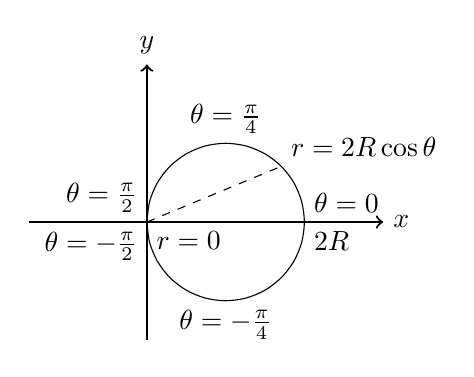
\begin{tikzpicture}
			\draw[thick,->] (-1.5,0) -- (3,0) node[anchor=west]{$x$};
			\draw[thick,->] (0,-1.5) -- (0,2) node[anchor=south]{$y$};
			\draw[scale=1,domain=-pi/2:pi/2,smooth,variable=\x] plot ({2*cos(deg(\x))*cos(deg(\x))},{2*cos(deg(\x))*sin(deg(\x))});
			\draw (2,0) node[anchor=south west]{$\theta=0$} node[anchor=north west]{$2R$};
			\draw (1,1) node[anchor=south]{$\theta=\frac{\pi}{4}$};
			\draw (0,0) node[anchor=south east]{$\theta=\frac{\pi}{2}$};
			\draw (1,-1) node[anchor=north]{$\theta=-\frac{\pi}{4}$};
			\draw (0,0) node[anchor=north east]{$\theta=-\frac{\pi}{2}$};
			\draw[dashed] (0,0) node[anchor=north west]{$r=0$} -- ({2*cos(deg(pi/8))*cos(deg(pi/8))},{2*cos(deg(pi/8))*sin(deg(pi/8))}) node[anchor=south west]{$r=2R\cos\theta$};
		\end{tikzpicture}
	\end{center}
	The curve is a circle, as we can see, with $-\frac{\pi}{2} \leq \theta < \frac{\pi}{2}$
	\begin{align}
		\text{Charge } = \iint_{\text{circle}}\sigma\,dA &= \sigma_0\int^{\theta=\frac{\pi}{2}}_{\theta=-\frac{\pi}{2}}\int^{r=2R\cos\theta}_{0} \frac{r}{R}\sin^4\theta\,r\,dr\,d\theta \\
		&=\frac{8\sigma_0R^2}{3}\int^{\theta=\frac{\pi}{2}}_{\theta=-\frac{\pi}{2}}\cos^3\theta\,\sin^4\theta\,d\theta\\
		&=\frac{8\sigma_0R^2}{3}\int^{\sin\theta=1}_{\sin\theta=-1}\sin^4\theta-\sin^6\theta\,d\sin\theta \\
		&=\frac{8\sigma_0R^2}{3}(\frac{2}{5}-\frac{2}{7}) \\
		&=\frac{32\sigma_0R^2}{105}
	\end{align}
\end{solution}

\question Suppose that the height of a certain hill (in feet) is given by
\begin{equation*}
	h(x,y) = 10(2xy - 3x^2 - 4y^2 + 14x + 10y + 40),
\end{equation*}
where $x$ is the distance (in km) east, $y$ the distance north of the closest town
\begin{parts}
	\part Where is the top of Sameer Hills located, and how high is it?
	\begin{solution}
		The top of Sameer hills will correspond to a maxima of $h(x,y)$. And we know that $\nabla h=\vec{0}$ at the maxima. So we need to find points satisfying $\nabla h=\vec{0}$.
		\begin{align}
			\nabla h &= \frac{\partial h}{\partial x}\,\hat{\imath} + \frac{\partial h}{\partial y}\,\hat{\jmath} \\
			&= 10(2y-6x+14)\,\hat{\imath} + 10(2x-8y+10)\,\hat{\jmath} \\
			\therefore \nabla h = 0 &\implies 2y-6x+14=0\text{; }2x-8y+10 = 0 \\
			\implies (x,y) &= (3,2)\\
			h(3,2) &= 710
		\end{align}
		So the top of Sameer hills is located $3$ km east and $2$ km north of the closest town, and it is at a height of $710$ feet
	\end{solution}

	\part How steep is the slope (in feet per km) at a point 1 km north and 1 km east of Hostel 16? In what direction is the slope steepest, at that point?
	\begin{solution}
		\begin{equation}
			\nabla h (1,1) = 100\,\hat{\imath}+40\,\hat{\jmath}
		\end{equation}
		So the steepness of the slope at $(1,1)$ is $|\nabla h(1,1)|=20\sqrt{29}$ and the slope is steepest at $\frac{\nabla h(1,1)}{|\nabla h(1,1)|}=\frac{1}{\sqrt{29}}(5\,\hat{\imath}+2\,\hat{\jmath})$
	\end{solution}
\end{parts}

\question The gradient operator $\nabla $ behaves like a vector in $\lq\lq$ some sense". For example, divergence of a curl ($\nabla.\nabla\times\vec{A}~=~0$)~ for any $\vec{A}$, may suggest that it is just like $\vec{A}.\vec{B}\times\vec{C}$  being zero if any two vectors are equal. Prove that $\nabla\times\nabla\times{\vec{F}} = \nabla(\nabla.\vec{F}) - \nabla^2{\vec{F}}$. To what extent does this look like the well known expansion of  $\vec{A}\times\vec{B}\times\vec{C}$ ?
\begin{solution}
	We will be using Einstein summation convention. According to this convention:
	\begin{enumerate}
		\item The whole term is summed over any index which appears \textbf{twice} in that term
		\item Any index appearing only once in the term in not summed over and must be present in both LHS and RHS
	\end{enumerate}
	Don't be confused by this. The convention only is to simply omit the $\sum$ symbol. You can mentally insert the $\sum$ symbol to make sense of what the summation will look like \\
	Now, as may have been done in the lectures:
	\begin{gather}
		\vec{A}\cdot\vec{B} = A_iB_i \\
		\vec{A}\times\vec{B} = \epsilon_{ijk}A_jB_k\,\hat{e_i}
	\end{gather}
	where $\hat{e_i}$ is the unit vector in $i$ direction \\
	When the $\sum$ symbol is reinserted, this simply means $\sum\limits_{i=x,y,z}\sum\limits_{j=x,y,z}\sum\limits_{k=x,y,z}\epsilon_{ijk}A_jB_k\hat{e_i}$ \\
	Now we will represent each component of $\nabla$, $\frac{\partial}{\partial i}$ by $\partial_i$,
	\begin{align}
		\nabla \times \left( \nabla \times \vec{F} \right) &= \epsilon_{ijk}\partial_j\left(\nabla\times\vec{F}\right)_k\,\hat{e_i} = \epsilon_{ijk}\epsilon_{klm}\partial_j\partial_lF_m\,\hat{e_i} = \epsilon_{kij}\epsilon_{klm}\partial_j\partial_lF_m\,\hat{e_i}\\
		&= (\delta_{il}\delta_{jm}-\delta_{im}\delta_{jl})\partial_j\partial_lF_m\,\hat{e_i} \text{\,\,\,\,\,\,\,\,\,\,\,\,\,\,\,\,\,\,\,\,\,\,\,\,\,\,\,\,\,\,\,\,\,\,\,\,($\because \epsilon_{ijk}\epsilon{ilm} = \delta_{jl}\delta_{km} - \delta{jm}\delta{kl}$)} \\
		&= (\partial_m\partial_iF_m - \partial_l\partial_lF_i)\,\hat{e_i} \text{\,\,\,\,\,\,\,\,\,\,\,\,\,\,\,\,\,\,\,\,\,\,\,\,\,\,\,\,\,\,\,\,\,\,\,\,\,\,\,\,\,\,\,\,\,\,\,\,($\because \delta_{ij}A_j = A_i$)}\\
		&= \partial_i(\partial_mF_m)\,\hat{e_i} - \partial_l\partial_l(F_i\,\hat{e_i}) \\
		&= \nabla(\nabla\cdot\vec{F})-\nabla^2\vec{F} \hskip0.55\textwidth\blacksquare
	\end{align}
	We know that $\vec{A}\times\vec{B}\times\vec{C} = \vec{B}(\vec{A}\cdot\vec{C}) - (\vec{A}\cdot\vec{B})\vec{C}$. If we write $\vec{A}=\nabla$, $\vec{B}=\nabla$, $\vec{C}=\vec{F}$, we get $\nabla\times\nabla\times\vec{F} = \nabla(\nabla\cdot\vec{F}) - (\nabla\cdot\nabla)\vec{F} = \nabla(\nabla\cdot\vec{F})-\nabla^2\vec{F}$. So this serves as a fake proof of the identity
\end{solution}

\end{questions}
\end{document}